\documentclass[10pt,a4paper]{article}
\usepackage[utf8]{inputenc}
\usepackage{amsmath}
\usepackage{amsfonts}
\usepackage{amssymb}
\usepackage{natbib}
\usepackage{graphicx}

\title{XOR single-layer model theory}
\author{Max Cotton}
\date{}

\begin{document}

\maketitle

\section{Setup}

\begin{figure}[h!]
\centering
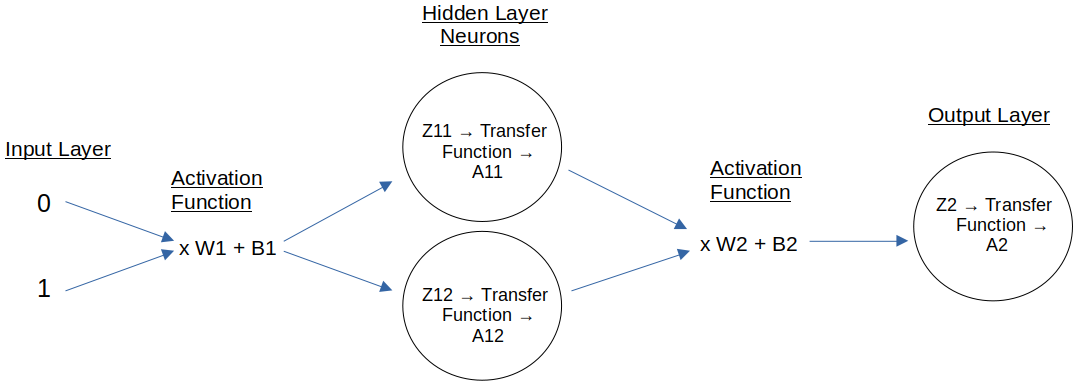
\includegraphics[width=1\textwidth]{src/images/xor-ann-diagram.png}
\end{figure}

\begin{itemize}
    \item Where W1 is the array of hidden weights, initially given random values, and B1 is the array of hidden biases, initially set to zeros
    \item Z11 and Z12 are together in an array Z1, and is the dot product of the W1 array and the input array (X) summed with the B1 array
    \item A11 and A12 are together in an array A1, and is sigmoid(Z1)
    \begin{itemize}
        \item Where $sigmoid(Z) = \frac{1}{1+e^{-Z}}$
    \end{itemize}
    \item W2 is the array of output weights, initially given random values, and B2 is the array of output biases, initially set to zeros
    \item Z2 is the dot product of the W2 array and A1 summed with the B2 array
    \item A2 is sigmoid(Z2), which is the prediction
\end{itemize}

\section{Forward Propagation}
For each epoch the input array consisting of a combination of a 0 and/or 1, is fed through the network to obtain a prediction A2

\section{Back Propagation}

\begin{itemize}
    \item Once a prediction is obtained, you then move back through the network adjusting the weights and biases
    \item The "Loss" (L) (how wrong the prediction is) can be calculated with the Loss function, which calculates the average difference between the prediction (A2) and the actual value (Y), the average is found by summing the result for each prediction then dividing by the number of predictions (m). This shows how well the network is performing.
    \begin{itemize}
        \item Where $L = -(\frac{1}{m}) * \sum(Y * log(A2) + (1-Y) * log(1-A2))$ and "log()" is the natural logarithm (e is the base)
    \end{itemize}
    \item Weights and biases are adjusted via Gradient Descent, which aims to get the minimum Loss value, with the following formula:
    \begin{itemize}
        \item $W = W - learningRate * \frac{\partial{L}}{\partial{W}}$
        \begin{itemize}
            \item Where $\frac{\partial{L}}{\partial{W2}} = (A2-Y) * A1$
            \item And $\frac{\partial{L}}{\partial{W1}} = X * A1 * (1-A1) * W2 * (A2-Y)$
        \end{itemize}
        \item $B = B - learningRate * \frac{\partial{L}}{\partial{B}}$
        \begin{itemize}
            \item Where $\frac{\partial{L}}{\partial{B2}} = A2-Y$
            \item And $\frac{\partial{L}}{\partial{B1}} = A1 * (1-A1) * W2 * (A2-Y)$
        \end{itemize}
    \end{itemize}
\end{itemize}

\section{Derivations for $\frac{\partial{L}}{\partial{W2}}$, $\frac{\partial{L}}{\partial{B2}}$ and $\frac{\partial{L}}{\partial{W1}}$, $\frac{\partial{L}}{\partial{B1}}$}

\begin{itemize}
    \item Functions used so far:
    \begin{enumerate}
        \item $Z1 = W1 . X + B1$
        \item $A1 = \frac{1}{1+e^{-Z1}}$
        \item $Z2 = W2 . A1 + B2$
        \item $A2 = \frac{1}{1+e^{-Z2}}$
        \item $L = -(\frac{1}{m}) * \sum(Y * log(A2) + (1-Y) * log(1-A2))$
    \end{enumerate}
    \item $\frac{\partial{L}}{\partial{W2}}$ derivation:
    \begin{itemize}
        \item By the Chain rule, $\frac{\partial{L}}{\partial{W2}} = \frac{\partial{L}}{\partial{A2}} * \frac{\partial{A2}}{\partial{Z2}} * \frac{\partial{Z2}}{\partial{W2}}$
        \item Using function 5, $\frac{\partial{L}}{\partial{A2}} = (-\frac{1}{m})(\frac{Y-A2}{A2(1-A2)})$
        \item Using function 4, $\frac{\partial{A2}}{\partial{Z2}} = A2 * (1-A2)$
        \item Using function 3, $\frac{\partial{Z2}}{\partial{W2}} = A1$
        \item => $\frac{\partial{L}}{\partial{W2}} = (-\frac{1}{m})(\frac{Y-A2}{A2(1-A2)}) * A2 * (1-A2) * A1\\
              = (A2-Y) * A1$
    \end{itemize}
    \item $\frac{\partial{L}}{\partial{B2}}$ derivation:
    \begin{itemize}
        \item By the Chain rule, $\frac{\partial{L}}{\partial{B2}} = \frac{\partial{L}}{\partial{A2}} * \frac{\partial{A2}}{\partial{Z2}} * \frac{\partial{Z2}}{\partial{B2}}$
        \item Using function 5, $\frac{\partial{L}}{\partial{A2}} = (-\frac{1}{m})(\frac{Y-A2}{A2(1-A2)})$
        \item Using function 4, $\frac{\partial{A2}}{\partial{Z2}} = A2 * (1-A2)$
        \item Using function 3, $\frac{\partial{Z2}}{\partial{B2}} = 1$
        \item => $\frac{\partial{L}}{\partial{B2}} = (-\frac{1}{m})(\frac{Y-A2}{A2(1-A2)}) * A2 * (1-A2)\\
              = A2-Y$
    \end{itemize}
    \item $\frac{\partial{L}}{\partial{W1}}$ derivation:
    \begin{itemize}
        \item By the Chain rule, $\frac{\partial{L}}{\partial{W1}} = \frac{\partial{A1}}{\partial{Z1}} * \frac{\partial{Z1}}{\partial{W1}} * \frac{\partial{L}}{\partial{Z2}} * \frac{\partial{Z2}}{\partial{A1}}$
        \item Using function 2, $\frac{\partial{A1}}{\partial{Z1}} = A1 * (1-A1)$
        \item Using function 1, $\frac{\partial{Z1}}{\partial{W1}} = X$
        \item Using function 5, $\frac{\partial{L}}{\partial{Z2}} = A2 - Y$
        \item Using function 3, $\frac{\partial{Z2}}{\partial{A1}} = W2$
        \item => $\frac{\partial{L}}{\partial{W1}} = X * A1 * (1-A1) * W2 * (A2-Y)$
    \end{itemize}
    \item $\frac{\partial{L}}{\partial{B1}}$ derivation:
    \begin{itemize}
        \item By the Chain rule, $\frac{\partial{L}}{\partial{W1}} = \frac{\partial{A1}}{\partial{Z1}} * \frac{\partial{Z1}}{\partial{B1}} * \frac{\partial{L}}{\partial{Z2}} * \frac{\partial{Z2}}{\partial{A1}}$
        \item Using function 2, $\frac{\partial{A1}}{\partial{Z1}} = A1 * (1-A1)$
        \item Using function 1, $\frac{\partial{Z1}}{\partial{B1}} = 1$
        \item Using function 5, $\frac{\partial{L}}{\partial{Z2}} = A2 - Y$
        \item Using function 3, $\frac{\partial{Z2}}{\partial{A1}} = W2$
        \item => $\frac{\partial{L}}{\partial{B1}} = A1 * (1-A1) * W2 * (A2-Y)$
    \end{itemize}
\end{itemize}

\end{document}